\usepackage{ifthen}

% Define an agenda item
%
% Arguments:
% 1: Identifier of the agenda item, should be all lower-case
% 2: Type of the agenda item: lecture or lab
% 3: English title of the agenda item
% 4: English full description of the agenda item
% 5: French title of the agenda item
% 6: French full description of the agenda item
\newcommand\defagendaitem[6]{
  \ifthenelse{\equal{\agendalanguage}{french}}{
    \expandafter\def\csname #1@#2@title\endcsname {#5}
    \expandafter\def\csname #1@#2@contents\endcsname {#6}
  }{
    \expandafter\def\csname #1@#2@title\endcsname {#3}
    \expandafter\def\csname #1@#2@contents\endcsname {#4}
  }
}

% Show/render an agenda item
%
% Arguments:
% 1: Identifier of the agenda item, as defined by \defagendaitem
% 2: Type of the agenda item: lecture or lab
\newcommand\showagendaitem[2]{%
  \ifthenelse{\boolean{hlineneeded}}{\\\hline}{\setboolean{hlineneeded}{true}}%
    \ifthenelse{\equal{\agendalanguage}{french}}{%
      \ifthenelse{\equal{#2}{lecture}}%
      {Cours &}%
      {%
        \ifthenelse{\equal{#2}{lab}}{%
          \ifthenelse{\equal{\trainingtype}{online}}{Démo &}{TP &}%
        }%
        {}%
      }%
    }{%
      \ifthenelse{\equal{#2}{lecture}}%
      {Lecture &}%
      {%
        \ifthenelse{\equal{#2}{lab}}{%
          \ifthenelse{\equal{\trainingtype}{online}}{Demo &}{Lab &}%
        }%
        {}%
      }%
    }%
    \csname #1@#2@title\endcsname &%
    \vspace{-12pt}%
    \csname #1@#2@contents\endcsname%
}%

% Define a board
%
% Arguments:
% 1: Identifier for the board, must be all lower-case
% 2: English title
% 3: English full description
% 4: French title
% 5: French full description
% 6: Board picture
\newcommand\defboard[6]{
  \ifthenelse{\equal{\agendalanguage}{french}}{
    \expandafter\def\csname #1@title\endcsname {#4}
    \expandafter\def\csname #1@contents\endcsname {#5}
  }{
    \expandafter\def\csname #1@title\endcsname {#2}
    \expandafter\def\csname #1@contents\endcsname {#3}
  }
  \expandafter\def\csname #1@image\endcsname {#6}
}

% Show/render a board
%
% Arguments:
% 1: Identifier of the board, as defined by \defboard
\newcommand\showboarditem[1]{
  \begin{tabularx}{\textwidth}{p{7cm}p{11cm}}
    \arrayrulecolor{blorange}
    \hline
    \multicolumn{1}{l}{\textbf{\textcolor{blorange}{\large \csname #1@title\endcsname}}} & \\
    \hline
    \arrayrulecolor{gray}
    \csname #1@contents\endcsname &
    \csname #1@image\endcsname \\
  \end{tabularx}
}

% Start an agenda by finding
% out if it is a morning or an
% afternoon if the training
% takes place on site
%
% Arguments:
% 1: Number of the half-day
\newcommand\showagendaday[1]{%
  \arrayrulecolor{blorange}%
  \\\hline%
  \multicolumn{3}{l}{%
    \textbf{\textcolor{blorange}{\large%
      \ifthenelse{\equal{\trainingtype}{online}}{%
        \showonlineagendaday{#1}%
      }{%
        \pgfmathparse{int(mod(#1, 2))}%
        \ifnum\pgfmathresult=1%
          \pgfmathparse{int((#1 + 1) / 2)}%
          \showonsiteagendaday{\pgfmathresult}{morning}%
        \else%
          \pgfmathparse{int(#1 / 2)}%
          \showonsiteagendaday{\pgfmathresult}{afternoon}%
        \fi%
      }%
    }}%
  } \\%
  \hline%
  \setboolean{hlineneeded}{false}%
  \arrayrulecolor{gray}%
}%

% Start an online agenda half-day
%
% Arguments:
% 1: Number of the half-day
\newcommand\showonlineagendaday[1]{%
  \ifthenelse{\equal{\agendalanguage}{french}}{%
    Demi-journée #1%
  }{%
    Half day #1%
  }%
}%

% Start an on-site agenda half-day
%
% Arguments:
% 1: Number of the day
% 2: "morning" or "afternoon"
\newcommand\showonsiteagendaday[2]{%
  \ifthenelse{\equal{\agendalanguage}{french}}{%
    \ifthenelse{\equal{#2}{morning}}{%
      Jour #1 - Matin%
    }{%
      Jour #1 - Après-midi%
    }%
  }{%
    \ifthenelse{\equal{#2}{morning}}{%
      Day #1 - Morning%
    }{%
      Day #1 - Afternoon%
    }%
  }%
}%

\defboard
{stm32mp1}
{STM32MP1 Discovery Kit}
{
  One of these Discovery Kits from STMicroelectronics: {\bf
  STM32MP157A-DK1}, {\bf STM32MP157D-DK1}, {\bf STM32MP157C-DK2} or
  {\bf STM32MP157F-DK2}
  \begin{itemize}
  \item STM32MP157, dual Cortex-A7 processor from STMicroelectronics
  \item USB powered
  \item 512 MB DDR3L RAM
  \item Gigabit Ethernet port
  \item 4 USB 2.0 host ports
  \item 1 USB-C OTG port
  \item 1 Micro SD slot
  \item On-board ST-LINK/V2-1 debugger
  \item Arduino compatible headers
  \item Audio codec, buttons, LEDs
  \item LCD touchscreen (DK2 kits only)
  \vspace{-0.7cm}
  \end{itemize}
}
{Plateforme STM32MP1}
{
  Une de ces cartes de STMicroelectronics : {\bf
  STM32MP157A-DK1}, {\bf STM32MP157D-DK1}, {\bf STM32MP157C-DK2} ou
  {\bf STM32MP157F-DK2}
  \begin{itemize}
  \item Processeur STM32MP157, double Cortex-A7, de STMicroelectronics
  \item Alimentée par USB
  \item 512 Mo DDR3L RAM
  \item Port Gigabit Ethernet port
  \item 4 ports hôte USB 2.0
  \item 1 port USB-C OTG
  \item 1 connecteur Micro SD
  \item Debugger ST-LINK/V2-1 sur la carte
  \item Connecteurs compatibles Arduino Uno v3
  \item Codec audio
  \item Divers : boutons, LEDs
  \item Écran LCD tactile (uniquement sur cartes DK2)
  \vspace{-0.7cm}
  \end{itemize}
}
{
  \begin{center}
    \includegraphics[width=5cm]{../slides/discovery-board-dk1/discovery-board-dk1.png}
  \end{center}
}

\defagendaitem
{qna}
{misc}
{Questions and Answers}
{
  \begin{itemize}
  \item Questions and answers with the audience about the course topics
  \item Extra presentations if time is left, according what most
        participants are interested in.
  \end{itemize}
}
{Questions / réponses}
{
  \begin{itemize}
  \item Questions et réponses avec les participants à propos des sujets abordés.
  \item Présentations supplémentaires s'il reste du temps, en fonction des demandes
        de la majorité des participants.
  \end{itemize}
}


\defboard
{beagleboneblack}
{BeagleBone Black}
{
  {\bf BeagleBone Black} or {\bf BeagleBone Black Wireless} board
  \begin{itemize}
  \item An ARM AM335x (single Cortex-A8) processor from Texas
    Instruments
  \item USB powered
  \item 512 MB of RAM
  \item 2 or 4 GB of on-board eMMC storage
  \item USB host and device
  \item HDMI output
  \item 2 x 46 pins headers, to access UARTs, SPI buses, I2C buses
    and more.
  \item Ethernet or WiFi
  \end{itemize}
  \vspace{-0.7cm}
}
{BeagleBone Black}
{
  Carte {\bf BeagleBone Black} ou {\bf BeagleBone Black Wireless}
  \begin{itemize}
  \item Un processeur ARM AM335x de Texas Instruments (à base de
    Cortex-A8), avec accélération 3D, etc.
  \item 512 Mo de RAM
  \item 2 ou 4 Go de stockage eMMC
  \item USB hôte et device
  \item Sortie HDMI
  \item Connecteurs à 2 x 46 broches, pour accéder aux UARTs, aux bus
    SPI, aux bus I2C, et à d'autres entrées/sorties du processeur.
  \item Ethernet ou WiFi
  \vspace{-0.7cm}
  \end{itemize}
}
{
  \begin{center}
    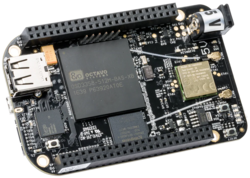
\includegraphics[width=5cm]{../slides/beagleboneblack-board/beagleboneblack_sd.png}
  \end{center}
}

\defboard
{beagleplay}
{BeaglePlay}
{
  {\bf BeaglePlay} board
  \begin{itemize}
    \item Texas Instruments AM625x (4xARM Cortex-A53 CPU)
    \item SoC with 3D acceleration, integrated MCU and many other peripherals.
    \item 2 GB of RAM
    \item 16 GB of on-board eMMC storage
    \item USB host and USB device, microSD, HDMI
    \item 2.4 and 5 GHz WiFi, Bluetooth and also Ethernet
    \item 1 MicroBus Header (SPI, I2C, UART, ...), OLDI and CSI connector.
  \vspace{-0.7cm}
  \end{itemize}
}
{BeaglePlay}
{
  Carte {\bf BeaglePlay}
  \begin{itemize}
    \item SoC Texas Instruments AM625x (CPU 4xARM Cortex-A53)
    \item SoC avec accélération 3D, MCU intégré et de nombreux autres périphériques.
    \item 2 GB de RAM
    \item 16 Go de stockage eMMC
    \item USB hôte et device, microSD, HDMI
    \item WiFi 2.4 and 5 GHz, Bluetooth et aussi Ethernet
    \item 1 Header MicroBus (SPI, I2C, UART, ...), connecteurs OLDI et CSI.
  \vspace{-0.7cm}
  \end{itemize}
}
{
  \begin{center}
    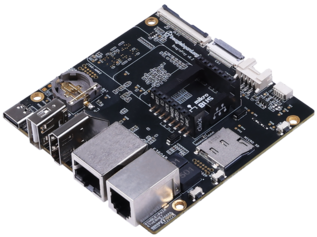
\includegraphics[width=5cm]{../slides/beagleplay-board/beagleplay_sd.png}
  \end{center}
}

\defboard
{espressobin}
{Hardware platform for practical labs}
{
  {\bf Globalscale EspressoBin} board
  \begin{itemize}
  \item Dual Cortex A53 Marvell Armada 3720 SoC
  \item Onboard switch with 2x 1Gbps interfaces
  \item Extra 1Gbps interface
  \item 1GB RAM
  \item 1x SATA interface
  \item 1x USB 3.0 interface
  \end{itemize}
}
{Plateforme matérielle pour les travaux pratiques}
{
  Carte {\bf Globalscale EspressoBin}
  \begin{itemize}
  \item SoC Marvell Armada 3720 SoC (CPU 2xARM Cortex A53)
  \item Switch Ethernet avec 2 interfaces Gigabit
  \item Interface Gigabit Ethernet additionnelle
  \item 1GB de RAM
  \item 1x interface SATA
  \item 1x interface USB 3.0
  \end{itemize}
}
{
  \begin{center}
    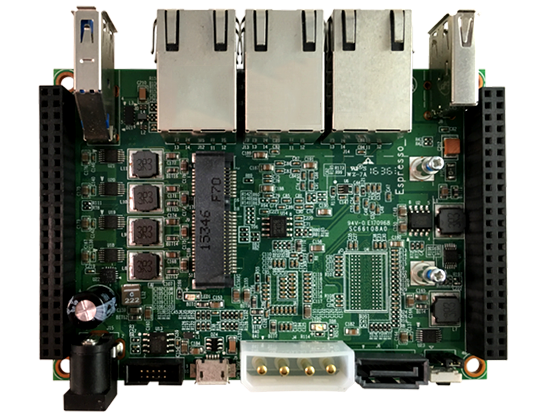
\includegraphics[width=5cm]{../slides/espressobin/espressobin.png}
  \end{center}
}


\def \inprogress{true}

\def \training{networking}

% Title
\ifthenelse{\equal{\agendalanguage}{french}}{
  \def \trainingtitle{Formation stack réseau sous Linux embarqué}
}{
  \def \trainingtitle{Embedded Linux Networking training}
}

% Duration
\ifthenelse{\equal{\trainingtype}{online}}{
  \def \trainingduration{4}
}{
  \def \trainingduration{3}
}

\def \trainingicon{common/flaticon-networking-training.png}

% Training objectives
\ifthenelse{\equal{\agendalanguage}{french}}{
  \def \traininggoals{
    \begin{itemize}
    \item Être capable de comprendre la pile réseau du noyau Linux
      dans son ensemble et de configurer des interfaces réseau
      complexes
    \item Être capable de comprendre le cheminement des paquets réseau
      dans un système Linux, d'utiliser différents types de sockets,
      de générer et de filtrer le trafic
    \item Être capable d'utiliser les technologies eBPF et XDP pour
      améliorer le traitement du trafic réseau
    \item Être capable de comprendre l'architecture des pilotes réseau
      du noyau Linux
    \item Être capable de comprendre comment les PHYs Ethernet et les
      switchs sont pris en charge dans le noyau Linux
    \item Être capable de diagnostiquer et de résoudre des problèmes
      liés au réseau bas niveau
    \end{itemize}
  }
}{
  \def \traininggoals{
    \begin{itemize}
    \item Be able to understand the overall Linux kernel networking
      stack and configure complex network devices
    \item Be able to understand the flow of network packets in a Linux
      system, use different socket types, generate and filter traffic
    \item Be able to use the eBPF and XDP technologies for improved
      network traffic processing
    \item Be able to understand the architecture of Linux kernel
      network drivers
    \item Be able to understand how Ethernet PHYs and switches are
      supported in the Linux kernel
    \item Be able to debug and troubleshoot low-level network related
      issues
    \end{itemize}
  }
}

% Training prerequisites
\def \trainingprerequisites{
  \begin{itemize}
    \prerequisiteembeddedlinux
    \prerequisitekernel
    \prerequisiteenglish
  \end{itemize}
}

% Training audience
\ifthenelse{\equal{\agendalanguage}{french}}{
  \def \trainingaudience{
    Ingénieurs travaillant sur le support réseau de systèmes Linux
    embarqués.
  }
}{
  \def \trainingaudience{
    Engineers working on networking support in Linux-based embedded
    devices
  }
}

\def \trainers {
  \ifthenelse{\equal{\agendalanguage}{french}}{
    Un des ingénieurs suivants
  }{
    One of the following engineers
  }\\
  \vspace{-12pt}
  \begin{itemize}
  \item \href{https://bootlin.com/company/staff/maxime-chevallier/}{Maxime Chevallier}
  \end{itemize}
}

% Time ratio
\def \onsitelecturetimeratio{50}
\def \onsitelabtimeratio{50}

\defagendaitem
{netdevices}
{lecture}
{Networking stack and network devices in Linux}
{
  \begin{itemize}
  \item Network stack overview in the linux kernel
  \item What is a network interface, overview of a \code{net_device}
  \item Overview of Ethernet, Wifi, CAN, Bluetooth, 802.15.4
  \item Stacked network devices and virtual network devices for VLAN,
    bridging, bonding
  \item Switchdev and DSA devices
  \item Control plane through {\em Netlink} and {\em ioctl}
  \end{itemize}
}
{Pile réseau et interfaces réseau dans Linux}
{
  \begin{itemize}
  \item Vue d'ensemble de la pile réseau dans le noyau Linux
  \item Qu'est-ce qu'une interface réseau, vue d'ensemble d'un \code{net_device}
  \item Vue d'ensemble d'Ethernet, Wifi, CAN, Bluetooth, 802.15.4
  \item Interfaces réseau {\em stackées} et interfaces réseau
    virtuelles pour le VLAN, le pontage, l'agrégation (bonding)
  \item Interfaces Switchdev et DSA
  \item Interface de contrôle via {\em Netlink} et {\em ioctl}
  \end{itemize}
}

\defagendaitem
{netdevices}
{lab}
{Setting up and configuring network interfaces}
{
  \begin{itemize}
  \item Basic setup with \code{iproute2}
  \item Create bridges, VLAN interfaces with \code{iproute2}
  \item Use network namespaces for interface isolation and testing
  \item Basic use of \code{tcpdump} and \code{wireshark}
  \item Using \code{ethtool} and \code{iproute2} to query the network
    interface features
  \end{itemize}
}
{Configuration et mise en place des interfaces réseau}
{
  \begin{itemize}
  \item Configuration de base avec \code{iproute2}
  \item Création de {\em bridges} et d'interfaces VLAN avec \code{iproute2}
  \item Utilisation des espaces de noms réseau ({\em network namespaces}) pour l'isolation et les tests des interfaces
  \item Utilisation de base de \code{tcpdump} et \code{wireshark}
  \item Utilisation de \code{ethtool} et \code{iproute2} pour interroger les fonctionnalités des interfaces réseau
  \end{itemize}
}

\defagendaitem
{packetpath}
{lecture}
{Path of a packet through the Linux networking stack}
{
  \begin{itemize}
  \item Discover the {\em Socket API}, the various families and types
    of sockets
  \item Sending and receiving data in userspace through sockets
  \item Using traffic generators and analysers in userspace with {\em
    Scappy} and {\em Wireshark}
  \item Path of a packet through the kernel, from a socket to a
    network driver
  \item Traffic filtering through {\em Netfilter} and \code{iptables}
  \item Traffic manipulation with the Traffic Control (\code{tc}) tool
  \item Queueing control with \code{tc} for performance optimisation
    and Time-Sensitive Networking (TSN)
  \end{itemize}
}
{Parcours d’un paquet à travers la pile réseau Linux}
{
  \begin{itemize}
  \item Découverte de l’{\em API Socket}, des différentes familles et
    types de sockets
  \item Envoi et réception de données en espace utilisateur via les
    sockets
  \item Utilisation de générateurs et analyseurs de trafic en espace
    utilisateur avec {\em Scapy} et {\em Wireshark}
  \item Parcours d’un paquet dans le noyau, d’un socket jusqu’à un
    pilote réseau
  \item Filtrage du trafic avec {\em Netfilter} et \code{iptables}
  \item Manipulation du trafic avec l’outil Traffic Control
    (\code{tc})
  \item Contrôle de l’ordonnancement (queueing) avec \code{tc} pour
    l’optimisation des performances et le {\em Time-Sensitive
      Networking} (TSN)
  \end{itemize}
}

\defagendaitem
{packetpath}
{lab}
{Sending and receiving traffic through sockets}
{
  \begin{itemize}
  \item Write a small tool using the various socket types
  \item Analyze the traffic through \code{wireshark} and \code{tcpdump}
  \item Filtering the traffic with {\em Netfilter} and \code{tc}
  \item Using traffic generators and performance measuring tools
  \end{itemize}
}
{Envoi et réception de trafic via les sockets}
{
  \begin{itemize}
  \item Écrire un petit outil utilisant les différents types de
    sockets
  \item Analyser le trafic avec \code{wireshark} et \code{tcpdump}
  \item Filtrer le trafic avec {\em Netfilter} et \code{tc}
  \item Utiliser des générateurs de trafic et des outils de mesure de
    performance
  \end{itemize}
}

\defagendaitem
{ebpf}
{lecture}
{eBPF for networking}
{
  \begin{itemize}
  \item Introduction to eBPF
  \item Compiling and loading eBPF programs
  \item BPF hooks in the networking stack
  \item Introduction to XDP
  \end{itemize}
}
{eBPF pour le réseau}
{
  \begin{itemize}
  \item Introduction à eBPF
  \item Compilation et chargement de programmes eBPF
  \item Points d'accroche BPF dans la pile réseau
  \item Introduction à XDP
  \end{itemize}
}

\defagendaitem
{ebpf}
{lab}
{Writing and using an XDP program}
{
  \begin{itemize}
  \item Write and load a simple XDP program to filter incoming traffic
  \item Use maps to configure the filter from userspace
  \end{itemize}
}
{Écriture et utilisation d’un programme XDP}
{
  \begin{itemize}
  \item Écrire et charger un programme XDP simple pour filtrer le
    trafic entrant
  \item Utiliser des maps pour configurer le filtre depuis l’espace
    utilisateur
  \end{itemize}
}

\defagendaitem
{netdrivers}
{lecture}
{Network device drivers}
{
  \begin{itemize}
  \item Overview of the hardware components and interfaces used in
    networking: MAC, PHY, MII, MDI, etc.
  \item Infrastructure of a typical Ethernet controller driver
  \item Sending and receiving packets with Napi
  \item Managing buffers and queues
  \item Packet timestamping for PTP
  \item Overview of {\em ethtool} driver operations for configuration
    and reporting
  \item Offloading network processing to the hardware
  \end{itemize}
}
{Pilotes de périphériques réseau}
{
  \begin{itemize}
  \item Vue d'ensemble des composants matériels et interfaces utilisés
    dans le réseau: MAC, PHY, MII, MDI, etc.
  \item Infrastructure d’un pilote typique de contrôleur Ethernet
  \item Envoi et réception de paquets avec Napi
  \item Gestion des tampons et des files d’attente
  \item Horodatage des paquets pour le PTP
  \item Vue d'ensemble des opérations de pilote {\em ethtool} pour la
    configuration et le diagnostic
  \item {\em Offloading} du traitement réseau vers le matériel
  \end{itemize}
}

\defagendaitem
{advancedethconfig}
{lab}
{Advanced Ethernet configuration}
{
  \begin{itemize}
  \item Investigating ethernet parameters controllable with {\em
    ethtool}
  \item Using the various offloading features
  \end{itemize}
}
{Configuration Ethernet avancée}
{
  \begin{itemize}
  \item Analyse des paramètres Ethernet configurables avec {\em
    ethtool}
  \item Utilisation des différentes fonctionnalités de déchargement
  \end{itemize}
}

\defagendaitem
{physwitch}
{lecture}
{Ethernet PHYs and switch support}
{
  \begin{itemize}
  \item Ethernet PHYs support in the kernel with {\em phylib}
  \item Interacting with PHYs through MDIO
  \item Dealing with the PHY to MAC connection with {\em phylink}
  \item Switch support through the {\em DSA} framework
  \item Dealing with switch operations with {\em switchdev}
  \end{itemize}
}
{Prise en charge des PHYs Ethernet et des switches}
{
  \begin{itemize}
  \item Prise en charge des PHYs Ethernet dans le noyau avec {\em phylib}
  \item Interaction avec les PHYs via MDIO
  \item Gestion de la connexion PHY vers MAC avec {\em phylink}
  \item Prise en charge des switches via le framework {\em DSA}
  \item Gestion de la configuration des switches avec {\em switchdev}
  \end{itemize}
}

\defagendaitem
{debugging}
{lecture}
{Network debugging and troubleshooting}
{
  \begin{itemize}
  \item Analyzing performances and packet drops with monitoring tools
  \item Debugging techniques for driver troubleshooting
  \item Using tracing tools and \code{perf} for performance analysis
  \item Diagnose hardware-related issues
  \end{itemize}
}
{Débogage et dépannage réseau}
{
  \begin{itemize}
  \item Analyse des performances et des pertes de paquets avec des
    outils de surveillance
  \item Techniques de débogage pour le dépannage des pilotes
  \item Utilisation des outils de traçage et de \code{perf} pour
    l’analyse des performances
  \item Diagnostic des problèmes liés au matériel
  \end{itemize}
}

\defagendaitem
{optimizing}
{lab}
{Optimizing the speed in various scenarios}
{
  \begin{itemize}
  \item Diagnosing and optimizing traffic speed
  \item Analyzing and troubleshooting latencies
  \end{itemize}
}
{Optimisation de la vitesse dans divers scénarios}
{
  \begin{itemize}
  \item Diagnostiquer et optimiser la vitesse du trafic
  \item Analyser et résoudre les problèmes de latence
  \end{itemize}
}

\def \agendaboards{espressobin}

\def \onlineagenda {
  \ifthenelse{\equal{\agendalanguage}{french}}{
    \section{Programme de la formation}
  }{
    \section{Training Schedule}
  }
  \begin{tabularx}{\textwidth}{p{2cm}p{5cm}p{11cm}}
  \showagendaday{1}
  \showagendaitem{netdevices}{lecture}
  \showagendaitem{netdevices}{lab}
  \showagendaitem{packetpath}{lecture}
  \showagendaday{2}
  \showagendaitem{packetpath}{lab}
  \showagendaitem{ebpf}{lecture}
  \showagendaitem{ebpf}{lab}
  \showagendaday{3}
  \showagendaitem{netdrivers}{lecture}
  \showagendaitem{advancedethconfig}{lab}
  \showagendaday{4}
  \showagendaitem{physwitch}{lecture}
  \showagendaitem{debugging}{lecture}
  \showagendaitem{optimizing}{lab}
  \end{tabularx}
}

\def \onsiteagenda {
  \ifthenelse{\equal{\agendalanguage}{french}}{
    \section{Programme de la formation}
  }{
    \section{Training Schedule}
  }
  \begin{tabularx}{\textwidth}{p{2cm}p{5cm}p{11cm}}
  \showagendaday{1}
  \showagendaitem{netdevices}{lecture}
  \showagendaitem{netdevices}{lab}
  \showagendaday{2}
  \showagendaitem{packetpath}{lecture}
  \showagendaitem{packetpath}{lab}
  \showagendaday{3}
  \showagendaitem{ebpf}{lecture}
  \showagendaitem{ebpf}{lab}
  \showagendaday{4}
  \showagendaitem{netdrivers}{lecture}
  \showagendaitem{advancedethconfig}{lab}
  \showagendaday{5}
  \showagendaitem{physwitch}{lecture}
  \showagendaday{6}
  \showagendaitem{debugging}{lecture}
  \showagendaitem{optimizing}{lab}
  \end{tabularx}
}
